\documentclass[dvipdfmx, 12pt]{beamer}
\usetheme{CambridgeUS}

\mode<presentation>

\begin{document}

\title{Event Representations for Automated Story Generation with Deep Neural Nets}
\author{竹下 颯太郎}
% \date[]{}
% \institute[a]{b}

\begin{frame}{}
\titlepage
\end{frame}


\section{はじめに}

\begin{frame}{AAAI 2018}
  \begin{figure}
    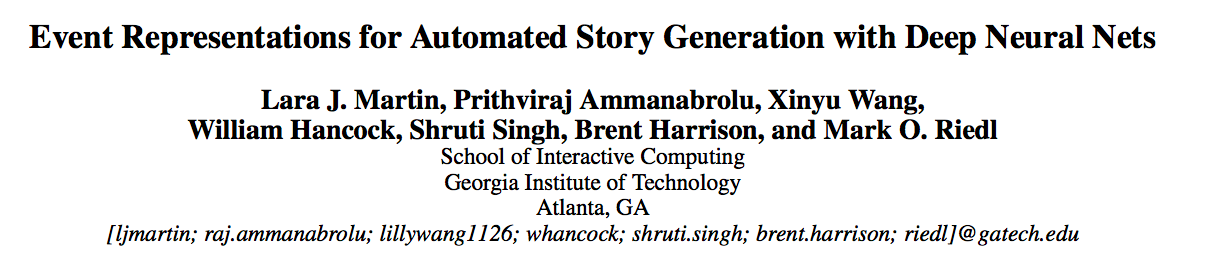
\includegraphics[width=1.0\textwidth]{imgs/paper.png}
  \end{figure}
\end{frame}

\begin{frame}{目的}
  \begin{itemize}
    \item 物語をニューラルネットワークを使用して生成したい.
    \item バラエティーに富んだ物語を,一貫性が壊れないように生成したい.
  \end{itemize}

  \begin{block}{この論文選択の理由}
    \begin{itemize}
      \item 技術的にすごい新しいわけではないが,タスクが面白い.
      \item が,難しすぎるからか,そこまで探索されている領域ではないので何かできるかもと思っている.
    \end{itemize}
  \end{block}
\end{frame}


\begin{frame}{目次}
\tableofcontents
\end{frame}


\section{背景}

\begin{frame}{背景}
  \begin{itemize}
    \item 複数の文からなる物語の生成は,一貫性の保持と柔軟性の確保の問題で難しい.
    \item 一貫性を保持しようと,ルールベースで頑張ると限界があるし,
    \item NNでいきなり生成しちゃうと,物語に一貫性がなくなる.
  \end{itemize}
  \begin{block}{問い}
    物語をいい感じの粒度で表現することで,一貫性と柔軟性の両方を担保できないか?
  \end{block}
\end{frame}


\section{提案手法}
\begin{frame}{提案手法 (俯瞰)}
  \begin{itemize}
    \item Event2Event (イベントの系列を生成する $\rightarrow$ Planning)
    \item Event2Sentence (Eventをhuman readableに変換)
  \end{itemize}
  \begin{figure}
    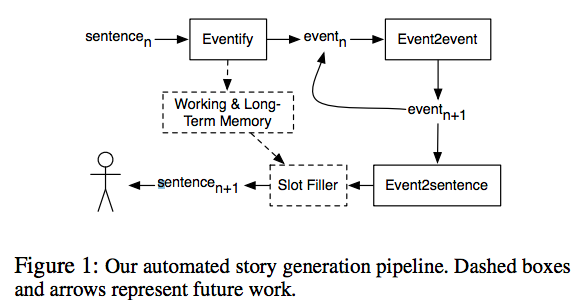
\includegraphics[width=0.6\textwidth]{imgs/framework.png}
  \end{figure}
\end{frame}

\begin{frame}{提案手法 (Eventの表現方法)}
    (s, v, o, m) $\rightarrow$ (subject, verb, object, modifier ("wildcord"))
  \begin{exampleblock}{例}
    "John and Mary went to the store" $\rightarrow$ (john, go store, $\phi$)と(mary, go, store, $\phi$)
  \end{exampleblock}
  Wikipediaのmovie plots corpusからStanford's CoreNLPを使用して,42,170 storiesからこの形式を抽出した.
\end{frame}

\begin{frame}{提案手法 (Event2Event)}
  \begin{itemize}
    \item 入力: $Event_{t}$
    \item 出力: $Event_{t+1}$
    \item モデル: Vanilla Multi layered RNN
  \end{itemize}

  \begin{alertblock}{自分の疑問}
    これRNNでやる意味あるのか?\\
    最初はてっきり,storyの時系列に対応するためにRNNを使用するのかと思った.
  \end{alertblock}
\end{frame}

\begin{frame}{提案手法 (Event2Sentence)}
  Event系列は前ステップで生成したが,human readableじゃないので,文に変換する必要がある.
  \begin{itemize}
    \item 入力: $Event_{t}$
    \item 出力: $Sentence_{t}$
    \item モデル: LSTM
  \end{itemize}
\end{frame}

\section{結果}
\begin{frame}{結果}
  \begin{figure}
    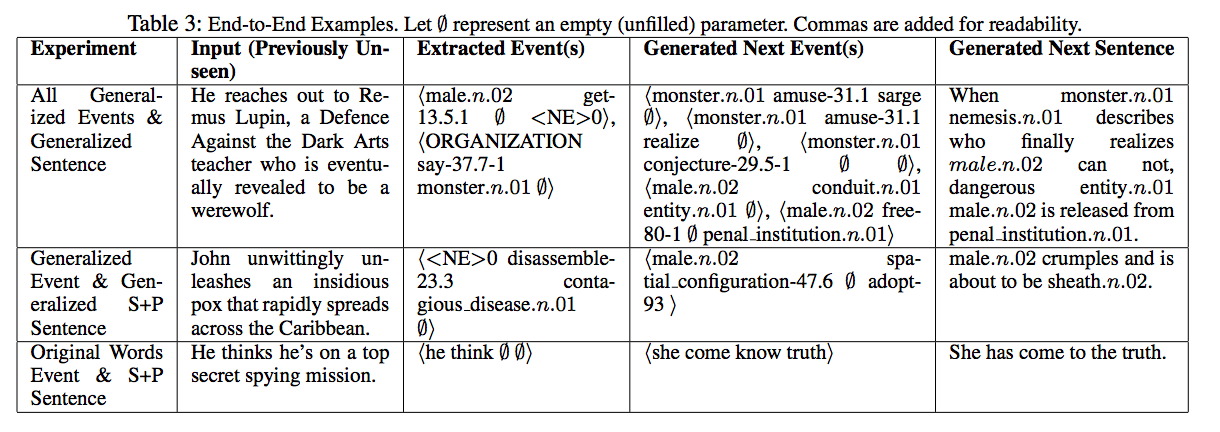
\includegraphics[width=1.0\textwidth]{imgs/result.png}
  \end{figure}
\end{frame}

\section{まとめ}
\begin{frame}{まとめ}
  \begin{itemize}
    \item 一貫性のある物語を,Event representationを経由させることで実現させようとした.
    \item 結果として,2つのRNNを使用することで,全自動で物語の生成をすることができた.
  \end{itemize}
\end{frame}

\end{document}
